\documentclass[11pt, a4paper]{article}
\usepackage[utf8]{inputenc}
\usepackage[T1]{fontenc}
\usepackage{helvet}
\renewcommand{\familydefault}{\sfdefault}
\usepackage[table]{xcolor}
\definecolor{schoolgreen}{HTML}{92D050}
\usepackage{geometry}
\geometry{margin=2cm, top=4cm, headheight=2.5cm, headsep=0.5cm}
\usepackage{array}
\usepackage{graphicx}
\usepackage{fancyhdr}
\usepackage{amssymb}

\pagestyle{fancy}
\fancyhf{}
\fancyhead[L]{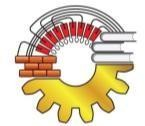
\includegraphics[height=2cm]{../../distritos/4117/templates/logo1.jpg}}
\fancyhead[R]{
\includegraphics[height=2cm]{../../distritos/4117/templates/logo2.jpg}}
\fancyhead[C]{\fontsize{10}{12}\selectfont \textbf{\textit{ESCUELA N.° 4-117 EJÉRCITO DE LOS ANDES \\ DIRECCIÓN DE EDUCACIÓN TÉCNICA Y TRABAJO \\ SECCIÓN V}}}
\renewcommand{\headrulewidth}{0pt}

\begin{document}

\noindent\colorbox{schoolgreen}{\begin{minipage}{\dimexpr\textwidth-2\fboxsep}\centering \textbf{\fontsize{14}{16}\selectfont DIAGNÓSTICO 2026}\end{minipage}}

\vspace{1.5em}

\begin{flushleft}
\textbf{Espacio Curricular:} Termodinámica y Máquinas Térmicas \\
\textbf{Año:} 5to \\
\textbf{División:} 2da \\
\textbf{Profesor/a:} Ferreyra Gustavo David \\
\textbf{Modalidad:} Electromecánica
\end{flushleft}

\vspace{1em}

\noindent \textbf{Marcar las capacidades a evaluar:}

\begin{itemize}
\item $\square$ Observación $\quad$ $\boxtimes$ Identificación $\quad$ $\square$ Comparación $\quad$ $\boxtimes$ Análisis
\item $\square$ Resumen $\quad$ $\square$ Síntesis $\quad$ $\boxtimes$ Clasificación $\quad$ $\boxtimes$ Interpretación
\item $\square$ Formulación de críticas $\quad$ $\square$ Búsqueda de suposiciones $\quad$ $\square$ Imaginación y creatividad
\item $\square$ Organización de datos $\quad$ $\square$ Formulación de hipótesis
\end{itemize}

\vspace{1em}

\noindent \textbf{1. Explicitar los aprendizajes específicos evaluados:}
\begin{itemize}
\item Conceptos básicos de calor, temperatura y energía interna.
\item Diferenciación entre procesos isotérmicos, isobáricos e isocóricos.
\item Conocimiento de las escalas termométricas y su conversión.
\item Nociones básicas sobre el funcionamiento de máquinas térmicas.
\end{itemize}

\noindent \textbf{2. Instrumento/s utilizado/s:}
\begin{itemize}
\item Cuestionario de preguntas abiertas y análisis de casos simples.
\item Prueba diagnóstica escrita con ejercicios de conversión de temperatura.
\end{itemize}

\noindent \textbf{3. Descripción de los destinatarios:}
El grupo se muestra participativo y con una curiosidad técnica elevada. Poseen una buena base de conceptos generales, aunque presentan dificultades en la formalización teórica y en la comprensión de conceptos abstractos como la entropía o la energía interna.

\noindent \textbf{4. Alumnos que presentan alguna dificultad:}

\begin{tabular}{|p{0.4\textwidth}|p{0.5\textwidth}|}
\hline
\rowcolor{gray!20} \textbf{Alumnos} & \textbf{Dificultad} \\
\hline
No se registran alumnos con dificultades significativas en esta etapa & N/A \\
\hline
\end{tabular}

\vspace{2em}

\noindent \textbf{Conclusión:}
De acuerdo a lo diagnosticado se podría decir que el grupo está apto para el desarrollo de la materia, sugiriendo un enfoque inicial basado en la experimentación práctica para anclar los conceptos teóricos abstractos de la termodinámica.

\end{document}